\documentclass[conference]{IEEEtran}
\IEEEoverridecommandlockouts
% The preceding line is only needed to identify funding in the first footnote. If that is unneeded, please comment it out.
\usepackage{cite}
\usepackage{amsmath,amssymb,amsfonts}
\usepackage{algorithmic}
\usepackage{algorithm}
\usepackage{graphicx}
\usepackage{textcomp}
\usepackage{courier}
\usepackage{xcolor}
\def\BibTeX{{\rm B\kern-.05em{\sc i\kern-.025em b}\kern-.08em
    T\kern-.1667em\lower.7ex\hbox{E}\kern-.125emX}}
\begin{document}

\title{Improving Join Reordering for SQL on Big Data Systems without Statistics\\
{\footnotesize \textsuperscript{*}Note: Sub-titles are not captured in Xplore and
should not be used}
\thanks{Identify applicable funding agency here. If none, delete this.}
}

\author{\IEEEauthorblockN{Amogh Margoor}
\IEEEauthorblockA{\textit{Qubole Inc} \\
Santa Clara, US}
\and
\IEEEauthorblockN{ Mayur Bhosale}
\IEEEauthorblockA{\textit{Qubole} \\
Bangalore, India}
}

\maketitle

\begin{abstract}
Traditional Cost Based Optimization in Query processing are not effective for SQL-on-Big Data due to lack of statistics. Statistics are mostly absent for Big Data Tables as they are both: expensive to compute and needs frequent recompute due to velocity of data change.  SQL Joins are common and critical for Analytics on Big Data; at Qubole we process around 4 million Joins just on Apache Spark in a month. Order in which joins are processed can significantly change the performance and efficiency of a workload. With lack of statistics traditional algorithms for reordering the Join are ineffective. Hence, we would like to propose a novel algorithm for Join Reordering which doesn't need expensive computation of Table statistics. We have observed it improving query performance by X.
\end{abstract}


\begin{IEEEkeywords}
component, formatting, style, styling, insert
\end{IEEEkeywords}

\section{Introduction}
Joins are extremely common for analytical workloads on Big Data. At Qubole, we offer 3 prominent SQL engines for Big Data as a service: Apache Hive, Presto and Apache Spark. Just in 1 month Qubole's offering of Apache Spark processed 4 million joins for our customers, making it one of the most commonly used SQL operators. Table \ref{tab:stats} specifies some of the Join metrics we collected for a month just for Apache Spark.

\begin{table}[h]
\begin{center}
\begin{tabular}{ |c|c| } 
 \hline
Joins Processed & 3.9 million \\ \hline
Most common Join Type & INNER JOIN - 51\%  \\ \hline
Second most common Join Type &  LEFT OUTER JOIN - 31\%\\ \hline
Most common Join algorithm & SortMergeJoin - 55\%\\ \hline
Second most common Join algorithm & BroadcastHashJoin - 44\%\\
 \hline
\end{tabular}
\caption{Join metrics collected over 1 month for Apache Spark in Qubole}
\label{tab:stats}
\end{center}
\end{table}

\subsection{Why is Join Reordering important ?}
All the prominent SQL Engines for Big Data like Apache SparkSQL, Presto, Hive etc  have Cost Based Join Reordering which give them multiple Xs in performance improvement\cite{b2}.

Let's look closely into how it can affect a query performance. For illustration, we will pick commonly used Join Algorithm in Presto and Apache Spark. Hash Join is commonly used distributed join in Presto and Sort Merge Join in Apache Spark.

\subsubsection{Distributed Hash Joins in Presto}

\begin{figure}[ht]
\centerline{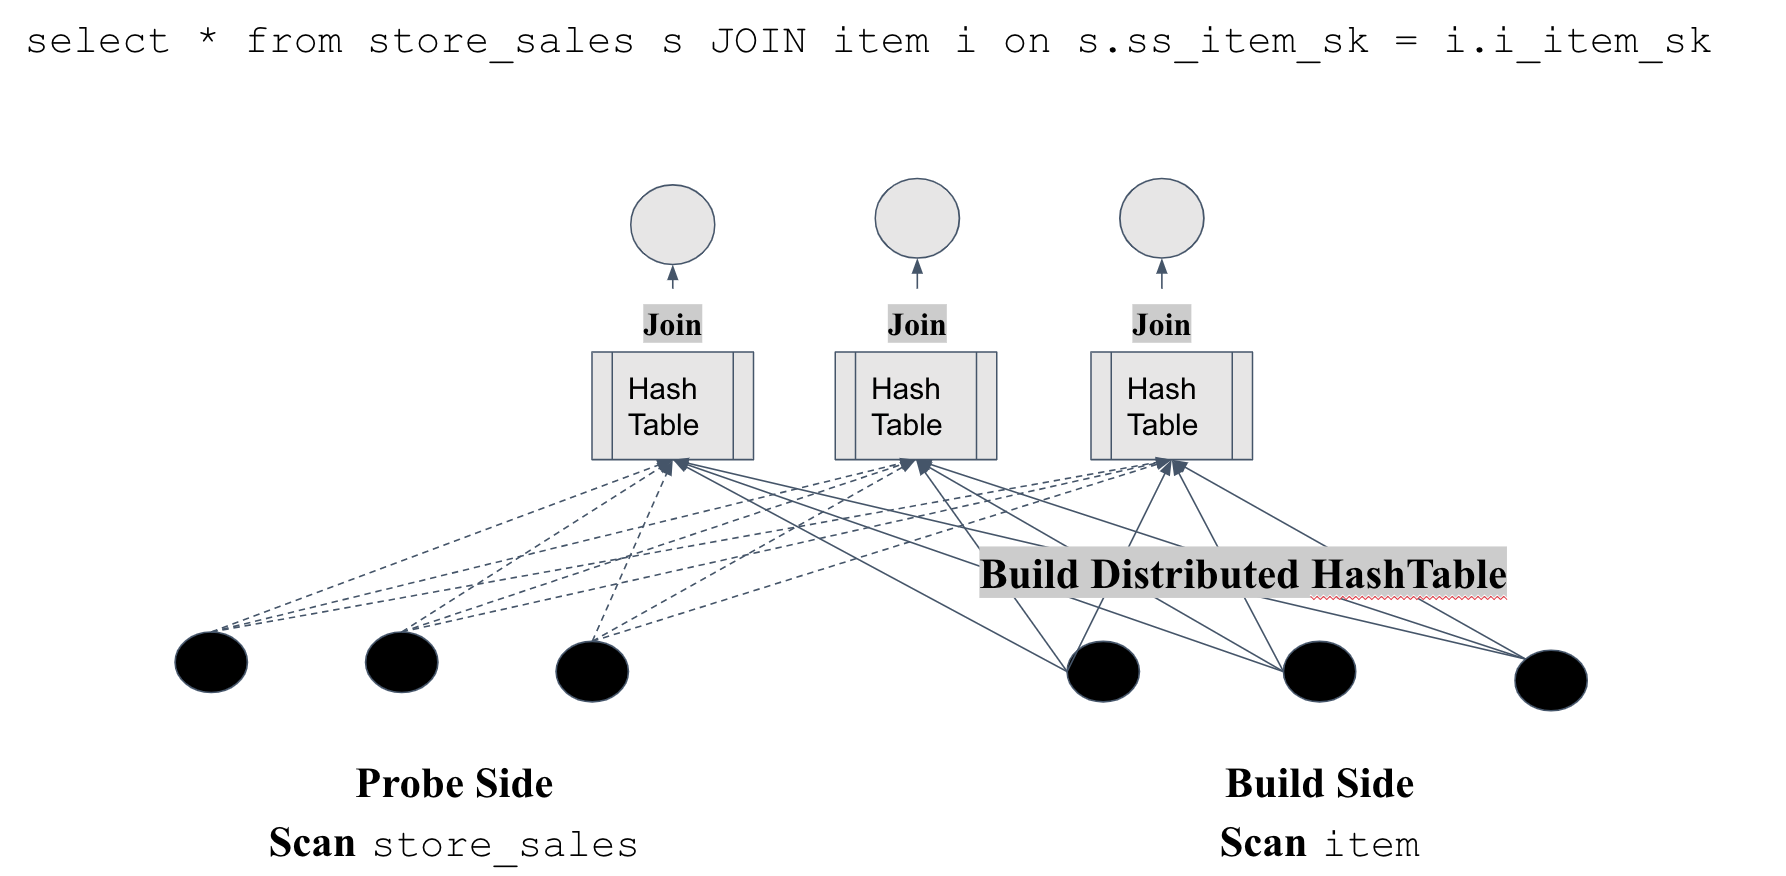
\includegraphics[width=9.5cm]{fig/DistributedHashJoin.png}}
\caption{Distributed Hash Join}
\label{distributed_hash_join}
\end{figure}

Hash Join is most commonly used distributed join algorithm in Presto.
Figure \ref{distributed_hash_join} illustrates this join.
When joining two tables \texttt{store\_sales} and \texttt{item} Presto regards table on the right i.e., \texttt{item}  as build side and table on left i.e., \texttt{store\_sales} as probe side.
Build side is used to build distributed hash table. As shown in the figure, after table \texttt{item} is scanned, its rows are hash distributed to different nodes based on join key \texttt{i\_item\_sk}. Once distributed, rows from table B are used to create Hash Table. Rows from the Probe Side are also distributed to different nodes using the same hash on the join key \texttt{i\_item\_sk}. Due to this partitioning \texttt{ss\_item\_sk}  and \texttt{i\_item\_sk} with same values end up in the same node.  Rows of Probe Side once distributed are checked against Hash table to find matching join rows. Here, major cost of the join will be building Hash tables on the Build Side. Hence, join reordering can considerably improve the performance by choosing smaller table as build side whenever possible (like in the cases of INNER Joins).

\subsubsection{Sort Merge Join in Spark}\label{subsubsec:sparkjoin}

\begin{figure}[ht]
\centerline{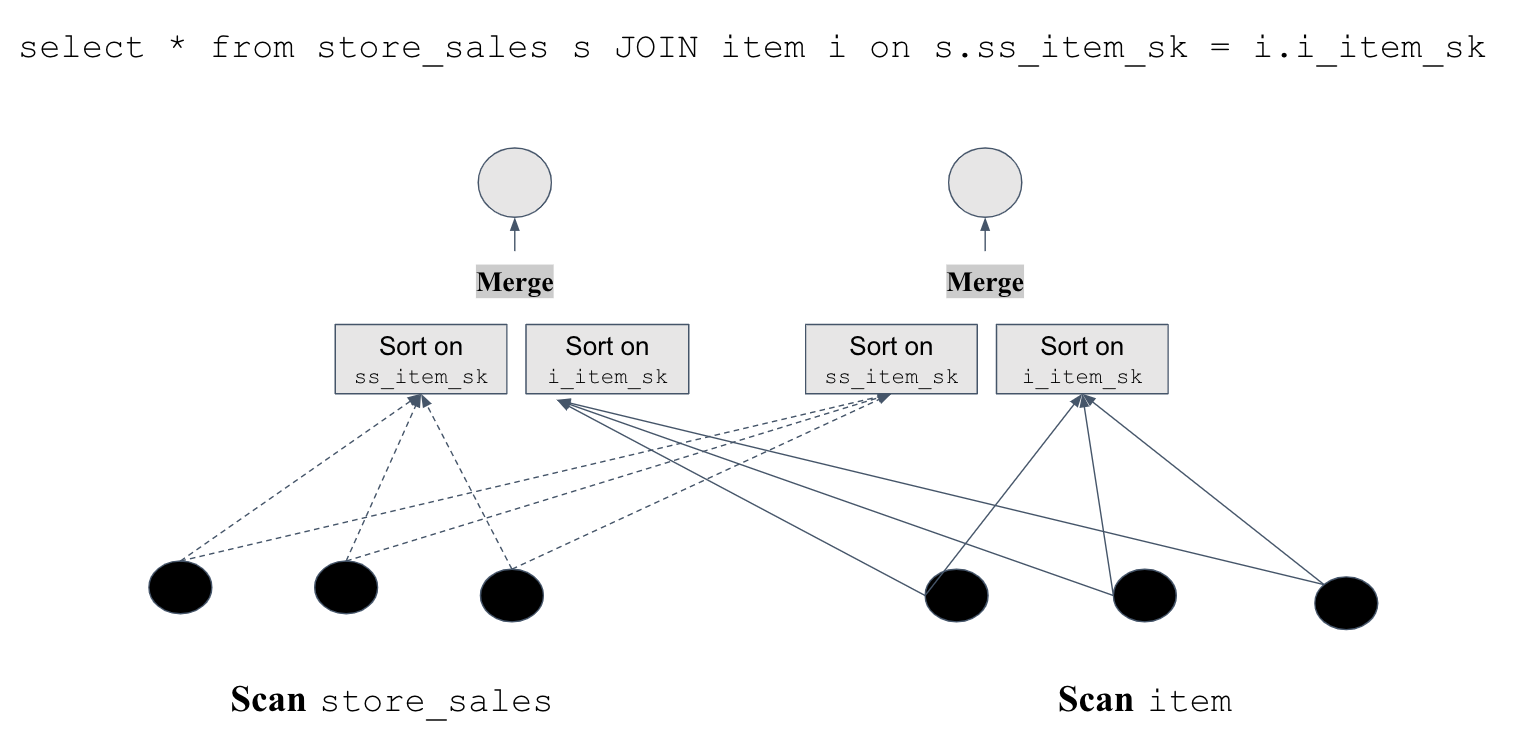
\includegraphics[width=9.5cm]{fig/SortMergeJoin.png}}
\caption{Sort Merge Join}
\label{sort_merge_join}
\end{figure}

Spark implements both Sort Merge Join and Hash Join.
Hash Joins are commonly used for Broadcast Joins, where if one of the sides of join is less in size than the threshold set by \texttt{$sql.autoBroadcastJoinThreshold$} then that side's hash table gets broadcasted to nodes with other larger side.
Join is performed locally on those nodes against the broadcasted hash table.

Except for the above case, Sort Merge Join is most commonly used join in Spark. Figure \ref{sort_merge_join} illustrates the Sort Merge Join.
Both tables \texttt{store\_sales} and \texttt{item} are distributed based on hash partitioning on join keys i.e., \texttt{ss\_item\_sk} and \texttt{i\_item\_sk} respectively. Due to this partitioning \texttt{ss\_item\_sk}  and \texttt{i\_item\_sk} with same values end up in the same node. Once rows from each table are distributed, they are individually sorted locally in every node and they are merged together to perform join. Internally Spark while doing merge uses scanner where for every key being considered for merging, one side will be streamed and another side will have rows with merge key buffered. Buffered rows can be spilled to disk too if it crosses memory threshold. In case of INNER Join, left side is streamed and right one will be buffered. So it is better to ensure the buffered side is the smaller one for lesser memory consumption and to avoid spill (spill can affect performance adversely). Hence, Join reordering is essential.

Both the above examples I provided were for a single join. In case of multi-way Join, reordering becomes even more important and can lead to huge performance improvements.
\subsection{Current State of Statistics and Join Reordering Algorithm for Big Data}

Currently, all these engines either use the Hive statistics or have statistics similar to it \cite{b1}:
\begin{itemize}
\item totalSize: Total size of the dataset as its seen at the filesystem level.
\item numFiles: Number of files the dataset consists of.
\item rawDataSize: Uncompressed size of the dataset.
\item numRows: Number of rows in the dataset.
\item columnStatistics: Statistics at column level: number of distinct values, max value, min value, number of null values, max length, average length.
\end{itemize}


\section{Related Work}

\section{Join Reordering without statistics}\label{sec:jo}
In the previous section we looked into the current state of affair for Join Reordering and why would it not work for Big Data systems. We will like to propose a novel approach in this section to reorder Join just based on the table sizes without any elaborate Table or Column Statistics as required by existing approaches.
We have implemented this approach in Apache Spark and will show how our approach gives up to X improvement in TPCDS queries in our empirical evaluation.

\subsection{Heuristics}

Let us look at the assumptions and heuristics used for the approach.

\subsubsection{Assumptions}\label{subsubsec:assumption}:

\begin{itemize}
\item In Star Schema Join, the Dimension table’s primary key will be joined with the Fact table’s foreign key.
\item Cardinality of Fact Table joined with Filtered Dimension table will be less than that of the Fact table.
\item So based on the last assumption, it follows that if Fact Join with Filtered Dimension happens earlier in multi-way join, it can benefit later joins.
\end{itemize}

To illustrate assumption above, let's look at this query:
\texttt{select * from fact\_table f join dim1 d1 on f.k1 = d1.pk join dim2 d2 on f.k2 = d2.pk where d2.date = ‘06-10-2019’}. If there is a filter on \texttt{dim2} which is smaller than \texttt{dim1} assumption is, it’s join with \texttt{fact\_table} would be smaller than \texttt{fact\_table}. Hence, joining \texttt{fact\_table} with \texttt{dim2} and then with \texttt{dim1} will be beneficial.

\subsubsection{Heuristics for detecting Star schema}
In the lack of relations information and statistics, we have to use only table sizes and query structure to determine if a Join is a start schema. We are using the following heuristics to determine them:

\begin{itemize}
\item Table involved in all of the joins should be a fact table.
\item At least half of the inner joins in the query should involve the fact table.
\item The ratio of the size of the largest dimensions table to fact table size should be lesser than a certain threshold.
\item None of the dimensions tables should be partitioned.
\end{itemize}

\subsubsection{Constraints for the Join Reorder algorithm}
We will define all the constraints or boundary conditions for the applicability of the algorithm here:

\begin{itemize}
\item \textbf{Star Schema Constraint}: Only Star schema Joins will be considered as assumptions made above are for Star Schema Join only.
\item \textbf{Simple Join Constraint}: Only INNER Joins whose left and right side are comprised of these operators that are deterministic and which do not increase the output size over the input size, other than Join.
\item \textbf{Shuffle Constraint}: For systems having shuffle like Spark or Hive, we reorder only if the number of shuffles do not increase due to it. For e.g., consider the following query: \texttt{select * from store\_sales s, item i, web\_sales ws, customer c where s.ss\_item\_sk = i.i\_item\_sk and i.i\_item\_sk = ws.i\_item\_sk and c.c\_customer\_sk = s.ss\_customer\_sk}
\item \textbf{Size Constraint}: Fact table should be at least $X$ times larger than dimension tables. $X$ is configurable.
\end{itemize}

\subsection{Algorithm}

\begin{algorithm}
\begin{algorithmic}[1]
\STATE  $\Omega$ $\gets$ $R_1$ $\Join$ $R_2$
\IF{$isStarSchemaJoin$($\Omega$) and $isSimpleJoin$($\Omega$) and $obeysShuffleConstraint$($\Omega$)}
    \STATE $type$ $\gets$ $treeType$($\Omega$) \COMMENT{$type$ will be either $left-deep$ or $right-deep$}
    \STATE ($\sigma$, $\delta$[$1$, $\ldots$, $n$]) $\gets$ $extractFactDimensions$($\Omega$)
    \STATE $\theta$[1, $\ldots$, k] $\gets$ $getFilteredDimensions$($\delta$[$1$, $\ldots$, $n$])
    \STATE $\pi$[1, $\ldots$, l] $\gets$ ($\delta$[$1$, $\ldots$, $n$] - $\theta$[1, $\ldots$, k]
    \STATE $\theta$[k+1] $\gets$ $dummyTable1$
    \STATE $dummyDim1$.$size$ $\gets$ $\infty$
    \STATE $\pi$[l+1] $\gets$ $dummyTable2$
    \STATE $dummyTable2$.$size$ $\gets$ $-\infty$
    \STATE $i$ $\gets$ 0
    \STATE $j$ $\gets$ 0
    \FOR{$r$ $\gets$ $1$ to $n$}
        \IF{$\theta$[$i$].size $\geq$ $\pi$[$j$].size}
            \STATE $i$ $\gets$ $i$ $+$ $1$
            \STATE $result$[$r$] $\gets$ $\theta$[$i$]
        \ELSE
            \STATE $j$ $\gets$ $j$ $+$ $1$
            \STATE $result$[$r$] $\gets$ $\pi$[$j$]
        \ENDIF
    \ENDFOR
    \STATE $\Omega$ $\gets$ $buildJoinTree$($type$, $\sigma$, $result$[$1$, $\ldots$, $n$])
\ENDIF
\RETURN $\Omega$
\end{algorithmic}
\label{algorithm}
\caption{Algorithm to Reorder Joins}
\end{algorithm}


In the algorithm presented above, $\Omega$ is assigned to the input Join that needs to be reordered. Following are the summary of steps to reorder them:
\begin{itemize}
\item Check if all constraints are satisfied for a join: \textbf{Star Schema Constraint}, \textbf{Simple Join Constraint}, \textbf{Shuffle Constraint}, \textbf{Size Constraint}.
\item Once it is a star schema, the Join tree can either be \textit{left-deep} or \textit{right-deep}. Obtain the information as we would like to construct reordered join the same way.
\item Extract the Fact table: $\sigma$ and Dimension tables: $ (\delta_1, \delta_2, \ldots, \delta_n)$. For dimension table, $\delta_i$ represents  $i^{th}$ dimension table being joined with the fact table $\sigma$ from the bottom of the Join Tree as shown in Figure \ref{left-deep}. As the tree here would be either \textit{left-deep} or \textit{right-deep} every dimension will have unique $i$ assigned to them.
\item Split dimensions into two lists: one with selective predicates. $\theta$ and another without it, $\pi$.
\item Sort the list with selective predicates i.e., $\theta$ based on sizes of the dimension tables. Sort the other list i.e., $\pi$ using user-provided order.
\item Merge both the list of dimensions by giving user order the preference for tables without a selective predicate, whereas for tables with selective predicates giving preference to smaller tables. When comparing the top of both the lists, if size of the top table in the selective predicate list is smaller than top of the other list, choose it otherwise vice-versa. This is in congruence with the Assumption made earlier in subsection \ref{subsubsec:assumption}.
\end{itemize}

\begin{figure}[ht]
\centerline{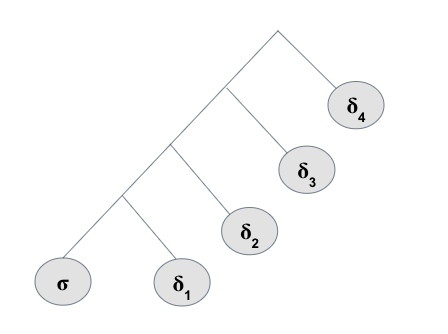
\includegraphics[width=5cm]{fig/left-deep.png}}
\caption{Left-Deep Tree with Fact table $\sigma$ and dimension tables $\delta_i$}
\label{left-deep}
\end{figure}


%\subsection{Maintaining the Integrity of the Specifications}

%The IEEEtran class file is used to format your paper and style the text. All margins, 
%column widths, line spaces, and text fonts are prescribed; please do not 
%alter them. You may note peculiarities. For example, the head margin
%measures proportionately more than is customary. This measurement 
%and others are deliberate, using specifications that anticipate your paper 
%as one part of the entire proceedings, and not as an independent document. 
%Please do not revise any of the current designations.
%
%\section{Prepare Your Paper Before Styling}
%Before you begin to format your paper, first write and save the content as a 
%separate text file. Complete all content and organizational editing before 
%formatting. Please note sections \ref{AA}--\ref{SCM} below for more information on 
%proofreading, spelling and grammar.
%
%Keep your text and graphic files separate until after the text has been 
%formatted and styled. Do not number text heads---{\LaTeX} will do that 
%for you.
%
%\subsection{Abbreviations and Acronyms}\label{AA}
%Define abbreviations and acronyms the first time they are used in the text, 
%even after they have been defined in the abstract. Abbreviations such as 
%IEEE, SI, MKS, CGS, ac, dc, and rms do not have to be defined. Do not use 
%abbreviations in the title or heads unless they are unavoidable.
%
%\subsection{Units}
%\begin{itemize}
%\item Use either SI (MKS) or CGS as primary units. (SI units are encouraged.) English units may be used as secondary units (in parentheses). An exception would be the use of English units as identifiers in trade, such as ``3.5-inch disk drive''.
%\item Avoid combining SI and CGS units, such as current in amperes and magnetic field in oersteds. This often leads to confusion because equations do not balance dimensionally. If you must use mixed units, clearly state the units for each quantity that you use in an equation.
%\item Do not mix complete spellings and abbreviations of units: ``Wb/m\textsuperscript{2}'' or ``webers per square meter'', not ``webers/m\textsuperscript{2}''. Spell out units when they appear in text: ``. . . a few henries'', not ``. . . a few H''.
%\item Use a zero before decimal points: ``0.25'', not ``.25''. Use ``cm\textsuperscript{3}'', not ``cc''.)
%\end{itemize}
%
%\subsection{Equations}
%Number equations consecutively. To make your 
%equations more compact, you may use the solidus (~/~), the exp function, or 
%appropriate exponents. Italicize Roman symbols for quantities and variables, 
%but not Greek symbols. Use a long dash rather than a hyphen for a minus 
%sign. Punctuate equations with commas or periods when they are part of a 
%sentence, as in:
%\begin{equation}
%a+b=\gamma\label{eq}
%\end{equation}
%
%Be sure that the 
%symbols in your equation have been defined before or immediately following 
%the equation. Use ``\eqref{eq}'', not ``Eq.~\eqref{eq}'' or ``equation \eqref{eq}'', except at 
%the beginning of a sentence: ``Equation \eqref{eq} is . . .''
%
%\subsection{\LaTeX-Specific Advice}
%
%Please use ``soft'' (e.g., \verb|\eqref{Eq}|) cross references instead
%of ``hard'' references (e.g., \verb|(1)|). That will make it possible
%to combine sections, add equations, or change the order of figures or
%citations without having to go through the file line by line.
%
%Please don't use the \verb|{eqnarray}| equation environment. Use
%\verb|{align}| or \verb|{IEEEeqnarray}| instead. The \verb|{eqnarray}|
%environment leaves unsightly spaces around relation symbols.
%
%Please note that the \verb|{subequations}| environment in {\LaTeX}
%will increment the main equation counter even when there are no
%equation numbers displayed. If you forget that, you might write an
%article in which the equation numbers skip from (17) to (20), causing
%the copy editors to wonder if you've discovered a new method of
%counting.
%
%{\BibTeX} does not work by magic. It doesn't get the bibliographic
%data from thin air but from .bib files. If you use {\BibTeX} to produce a
%bibliography you must send the .bib files. 
%
%{\LaTeX} can't read your mind. If you assign the same label to a
%subsubsection and a table, you might find that Table I has been cross
%referenced as Table IV-B3. 
%
%{\LaTeX} does not have precognitive abilities. If you put a
%\verb|\label| command before the command that updates the counter it's
%supposed to be using, the label will pick up the last counter to be
%cross referenced instead. In particular, a \verb|\label| command
%should not go before the caption of a figure or a table.
%
%Do not use \verb|\nonumber| inside the \verb|{array}| environment. It
%will not stop equation numbers inside \verb|{array}| (there won't be
%any anyway) and it might stop a wanted equation number in the
%surrounding equation.
%
%\subsection{Some Common Mistakes}\label{SCM}
%\begin{itemize}
%\item The word ``data'' is plural, not singular.
%\item The subscript for the permeability of vacuum $\mu_{0}$, and other common scientific constants, is zero with subscript formatting, not a lowercase letter ``o''.
%\item In American English, commas, semicolons, periods, question and exclamation marks are located within quotation marks only when a complete thought or name is cited, such as a title or full quotation. When quotation marks are used, instead of a bold or italic typeface, to highlight a word or phrase, punctuation should appear outside of the quotation marks. A parenthetical phrase or statement at the end of a sentence is punctuated outside of the closing parenthesis (like this). (A parenthetical sentence is punctuated within the parentheses.)
%\item A graph within a graph is an ``inset'', not an ``insert''. The word alternatively is preferred to the word ``alternately'' (unless you really mean something that alternates).
%\item Do not use the word ``essentially'' to mean ``approximately'' or ``effectively''.
%\item In your paper title, if the words ``that uses'' can accurately replace the word ``using'', capitalize the ``u''; if not, keep using lower-cased.
%\item Be aware of the different meanings of the homophones ``affect'' and ``effect'', ``complement'' and ``compliment'', ``discreet'' and ``discrete'', ``principal'' and ``principle''.
%\item Do not confuse ``imply'' and ``infer''.
%\item The prefix ``non'' is not a word; it should be joined to the word it modifies, usually without a hyphen.
%\item There is no period after the ``et'' in the Latin abbreviation ``et al.''.
%\item The abbreviation ``i.e.'' means ``that is'', and the abbreviation ``e.g.'' means ``for example''.
%\end{itemize}
%An excellent style manual for science writers is \cite{b7}.
%
%\subsection{Authors and Affiliations}
%\textbf{The class file is designed for, but not limited to, six authors.} A 
%minimum of one author is required for all conference articles. Author names 
%should be listed starting from left to right and then moving down to the 
%next line. This is the author sequence that will be used in future citations 
%and by indexing services. Names should not be listed in columns nor group by 
%affiliation. Please keep your affiliations as succinct as possible (for 
%example, do not differentiate among departments of the same organization).
%
%\subsection{Identify the Headings}
%Headings, or heads, are organizational devices that guide the reader through 
%your paper. There are two types: component heads and text heads.
%
%Component heads identify the different components of your paper and are not 
%topically subordinate to each other. Examples include Acknowledgments and 
%References and, for these, the correct style to use is ``Heading 5''. Use 
%``figure caption'' for your Figure captions, and ``table head'' for your 
%table title. Run-in heads, such as ``Abstract'', will require you to apply a 
%style (in this case, italic) in addition to the style provided by the drop 
%down menu to differentiate the head from the text.
%
%Text heads organize the topics on a relational, hierarchical basis. For 
%example, the paper title is the primary text head because all subsequent 
%material relates and elaborates on this one topic. If there are two or more 
%sub-topics, the next level head (uppercase Roman numerals) should be used 
%and, conversely, if there are not at least two sub-topics, then no subheads 
%should be introduced.
%
%\subsection{Figures and Tables}
%\paragraph{Positioning Figures and Tables} Place figures and tables at the top and 
%bottom of columns. Avoid placing them in the middle of columns. Large 
%figures and tables may span across both columns. Figure captions should be 
%below the figures; table heads should appear above the tables. Insert 
%figures and tables after they are cited in the text. Use the abbreviation 
%``Fig.~\ref{fig}'', even at the beginning of a sentence.
%
%\begin{table}[htbp]
%\caption{Table Type Styles}
%\begin{center}
%\begin{tabular}{|c|c|c|c|}
%\hline
%\textbf{Table}&\multicolumn{3}{|c|}{\textbf{Table Column Head}} \\
%\cline{2-4} 
%\textbf{Head} & \textbf{\textit{Table column subhead}}& \textbf{\textit{Subhead}}& \textbf{\textit{Subhead}} \\
%\hline
%copy& More table copy$^{\mathrm{a}}$& &  \\
%\hline
%\multicolumn{4}{l}{$^{\mathrm{a}}$Sample of a Table footnote.}
%\end{tabular}
%\label{tab1}
%\end{center}
%\end{table}

%\begin{figure}[htbp]
%\centerline{\includegraphics{fig1.png}}
%\caption{Example of a figure caption.}
%\label{fig}
%\end{figure}

%Figure Labels: Use 8 point Times New Roman for Figure labels. Use words 
%rather than symbols or abbreviations when writing Figure axis labels to 
%avoid confusing the reader. As an example, write the quantity 
%``Magnetization'', or ``Magnetization, M'', not just ``M''. If including 
%units in the label, present them within parentheses. Do not label axes only 
%with units. In the example, write ``Magnetization (A/m)'' or ``Magnetization 
%\{A[m(1)]\}'', not just ``A/m''. Do not label axes with a ratio of 
%quantities and units. For example, write ``Temperature (K)'', not 
%``Temperature/K''.

\section*{Acknowledgment}

%The preferred spelling of the word ``acknowledgment'' in America is without 
%an ``e'' after the ``g''. Avoid the stilted expression ``one of us (R. B. 
%G.) thanks $\ldots$''. Instead, try ``R. B. G. thanks$\ldots$''. Put sponsor 
%acknowledgments in the unnumbered footnote on the first page.

%\section*{References}

%Please number citations consecutively within brackets \cite{b1}. The 
%sentence punctuation follows the bracket \cite{b2}. Refer simply to the reference 
%number, as in \cite{b3}---do not use ``Ref. \cite{b3}'' or ``reference \cite{b3}'' except at 
%the beginning of a sentence: ``Reference \cite{b3} was the first $\ldots$''
%
%Number footnotes separately in superscripts. Place the actual footnote at 
%the bottom of the column in which it was cited. Do not put footnotes in the 
%abstract or reference list. Use letters for table footnotes.
%
%Unless there are six authors or more give all authors' names; do not use 
%``et al.''. Papers that have not been published, even if they have been 
%submitted for publication, should be cited as ``unpublished'' \cite{b4}. Papers 
%that have been accepted for publication should be cited as ``in press'' \cite{b5}. 
%Capitalize only the first word in a paper title, except for proper nouns and 
%element symbols.
%
%For papers published in translation journals, please give the English 
%citation first, followed by the original foreign-language citation \cite{b6}.

\begin{thebibliography}{00}
\bibitem{b1} Selinger, P. Griffiths, M. M., Astrahan, D. D., Chamberlin, R. A., Lorie, and T. G., Price. ``Access Path Selection in a Relational Database Management System.`` . In Proceedings of the 1979 ACM SIGMOD International Conference on Management of Data (pp. 23–34). Association for Computing Machinery, 1979.
\bibitem{b2} Amogh Margoor, Rajat Venkatesh. ``SQL Join Optimizations in Qubole Presto,``
https://medium.com/qubole-engineering/sql-join-optimizations-in-qubole-presto-3ced3dc75275, unpublished 
%\bibitem{b2} J. Clerk Maxwell, A Treatise on Electricity and Magnetism, 3rd ed., vol. 2. Oxford: Clarendon, 1892, pp.68--73.
%\bibitem{b3} I. S. Jacobs and C. P. Bean, ``Fine particles, thin films and exchange anisotropy,'' in Magnetism, vol. III, G. T. Rado and H. Suhl, Eds. New York: Academic, 1963, pp. 271--350.
%\bibitem{b4} K. Elissa, ``Title of paper if known,'' unpublished.
%\bibitem{b5} R. Nicole, ``Title of paper with only first word capitalized,'' J. Name Stand. Abbrev., in press.
%\bibitem{b6} Y. Yorozu, M. Hirano, K. Oka, and Y. Tagawa, ``Electron spectroscopy studies on magneto-optical media and plastic substrate interface,'' IEEE Transl. J. Magn. Japan, vol. 2, pp. 740--741, August 1987 [Digests 9th Annual Conf. Magnetics Japan, p. 301, 1982].
%\bibitem{b7} M. Young, The Technical Writer's Handbook. Mill Valley, CA: University Science, 1989.
\end{thebibliography}


%\vspace{12pt}
%\color{red}
%IEEE conference templates contain guidance text for composing and formatting conference papers. Please ensure that all template text is removed from your conference paper prior to submission to the conference. Failure to remove the template text from your paper may result in your paper not being published.

\end{document}
